%=================================================================
% CSE 4345 — Big Data Analytics
% Week 7, Part 2: Seminal Research & Case Study
% Department of CSE, Premier University
%
% SEMINAL PAPERS:
%   Thusoo et al. (2009) — Hive: A Warehousing Solution over a
%   Map-Reduce Framework. VLDB 2009. (cited >3,000 times)
%
%   Thusoo et al. (2010) — Hive: A Petabyte Scale Data Warehouse
%   Using Hadoop. IEEE ICDE 2010. (cited >1,500 times)
%
% CASE STUDY:
%   Spotify Discover Weekly (2015–2018) — Hive + Luigi + ColFilter
%   over 2 billion playlists for 30M weekly listeners
%=================================================================

\documentclass[aspectratio=169,10pt]{beamer}

%---------- Packages ----------
\usepackage[utf8]{inputenc}
\usepackage[T1]{fontenc}
\usepackage{booktabs}
\usepackage{xcolor}
\usepackage{tikz}
\usetikzlibrary{shapes.geometric, positioning, arrows.meta, decorations.pathreplacing}
\usepackage{amsmath}
\usepackage{graphicx}
\usepackage{multicol}
\usepackage{enumerate}
\usepackage{array}

%---------- Theme ----------
\usetheme{Madrid}

%---------- Premier University Color Identity ----------
\definecolor{PUNavy}{RGB}{10,36,99}
\definecolor{PUGold}{RGB}{197,151,37}
\definecolor{PULightBlue}{RGB}{210,228,255}
\definecolor{PUTeal}{RGB}{0,100,100}
\definecolor{PUGray}{RGB}{90,90,90}
\definecolor{PURed}{RGB}{160,30,30}
\definecolor{PUGreen}{RGB}{30,120,60}
\definecolor{PUPurple}{RGB}{90,30,120}
\definecolor{PUOrange}{RGB}{190,90,20}

\setbeamercolor{palette primary}{bg=PUNavy, fg=white}
\setbeamercolor{palette secondary}{bg=PUNavy!85, fg=white}
\setbeamercolor{palette tertiary}{bg=PUNavy!70, fg=white}
\setbeamercolor{palette quaternary}{bg=PUNavy, fg=white}
\setbeamercolor{structure}{fg=PUNavy}
\setbeamercolor{title}{bg=PUNavy, fg=PUGold}
\setbeamercolor{subtitle}{fg=white}
\setbeamercolor{frametitle}{bg=PUNavy, fg=PUGold}
\setbeamercolor{alerted text}{fg=PUGold!85!black}
\setbeamercolor{block title}{bg=PUNavy, fg=white}
\setbeamercolor{block body}{bg=PULightBlue!45}
\setbeamercolor{block title alerted}{bg=PUGold!80!black, fg=white}
\setbeamercolor{block body alerted}{bg=PUGold!12}
\setbeamercolor{block title example}{bg=PUTeal, fg=white}
\setbeamercolor{block body example}{bg=PUTeal!10}
\setbeamercolor{section in toc}{fg=PUNavy}
\setbeamercolor{itemize item}{fg=PUGold!80!black}
\setbeamercolor{itemize subitem}{fg=PUNavy!70}

\setbeamertemplate{navigation symbols}{}
\setbeamertemplate{itemize item}{\scriptsize\raise1.5pt\hbox{\textbullet}}
\setbeamertemplate{itemize subitem}{\scriptsize\raise1pt\hbox{--}}

%---------- Section separator ----------
\AtBeginSection[]{
  \begin{frame}[plain]
    \vfill
    \centering
    \begin{beamercolorbox}[sep=12pt,center,shadow=true,rounded=true]{block title}
      \usebeamerfont{title}\insertsectionhead\par
    \end{beamercolorbox}
    \vfill
  \end{frame}
}

%---------- Helper: citation box ----------
\newenvironment{paperbox}[1]{%
  \setbeamercolor{block title}{bg=PUNavy!90,fg=PUGold}
  \setbeamercolor{block body}{bg=PUNavy!6}
  \begin{block}{#1}}{%
  \end{block}}

%---------- Custom footline ----------
\setbeamertemplate{footline}{
  \leavevmode\hbox{%
    \begin{beamercolorbox}[wd=.333\paperwidth,ht=2.25ex,dp=1ex,center]{palette primary}
      \usebeamerfont{author in head/foot}\insertshortauthor
    \end{beamercolorbox}%
    \begin{beamercolorbox}[wd=.334\paperwidth,ht=2.25ex,dp=1ex,center]{palette secondary}
      \usebeamerfont{title in head/foot}\insertshorttitle
    \end{beamercolorbox}%
    \begin{beamercolorbox}[wd=.333\paperwidth,ht=2.25ex,dp=1ex,right]{palette primary}
      \usebeamerfont{date in head/foot}
      \insertframenumber{} / \inserttotalframenumber\hspace*{2ex}
    \end{beamercolorbox}}%
  \vskip0pt%
}

%---------- Title metadata ----------
\title[CSE 4345 \textbar{} Week 7, Part 2]{CSE 4345: Big Data Analytics}
\subtitle{Week 7, Part 2 \textemdash\ Seminal Research \& Case Study}
\author[Dept.\ of CSE]{Department of Computer Science \& Engineering\\[4pt]
       \small Premier University, Chittagong}
\institute{}
\date{Semester 2026}

%=================================================================
\begin{document}
%=================================================================

%----------------------------------------------------------------
% TITLE SLIDE
%----------------------------------------------------------------
\begin{frame}
  \titlepage
\end{frame}

%----------------------------------------------------------------
% PART 2 OVERVIEW
%----------------------------------------------------------------
\begin{frame}{Part 2 Overview — Week 7}
  \begin{columns}[T]
    \column{0.47\textwidth}
      \begin{block}{Today's Agenda}
        \tableofcontents
      \end{block}

    \column{0.50\textwidth}
      \begin{exampleblock}{Seminal Papers Covered}
        \begin{enumerate}
          \item Thusoo, A., et al. (2009).
                \textit{Hive: A Warehousing Solution over a
                Map-Reduce Framework.} VLDB 2009.
          \item Thusoo, A., et al. (2010).
                \textit{Hive: A Petabyte Scale Data Warehouse
                Using Hadoop.} IEEE ICDE 2010.
        \end{enumerate}
      \end{exampleblock}
      \vspace{6pt}
      \begin{alertblock}{Case Study}
        Spotify Discover Weekly (2015--2018):
        HiveQL + Luigi pipelines over \textbf{2 billion playlists}
        to generate personalised weekly mixes for
        \textbf{30 million} listeners.
      \end{alertblock}
      \vspace{4pt}
      \begin{block}{CLO Addressed}
        \textbf{CLO3, CLO4} — Explain SQL-on-Hadoop; solve
        petabyte-scale analytics design problems\\
        \textbf{PLO(b,c)}
      \end{block}
  \end{columns}
\end{frame}

%================================================================
\section{Paper 1 — Thusoo et al.\ (2009): Hive at VLDB}
%================================================================

%----------------------------------------------------------------
\begin{frame}{Research Landscape: SQL-on-Hadoop Timeline}
  \begin{center}
  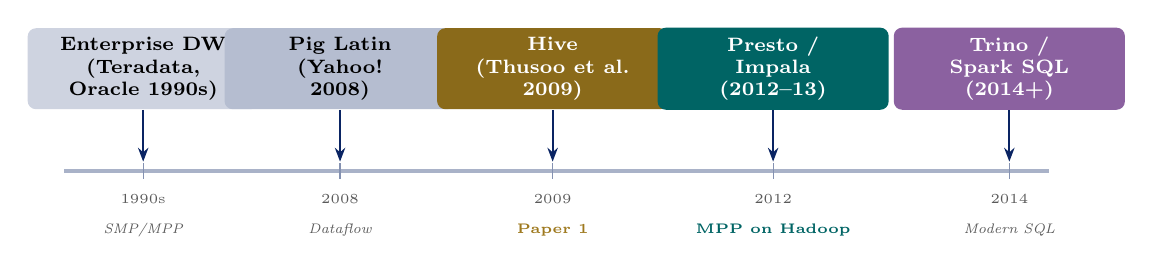
\begin{tikzpicture}[
      nbox/.style={rectangle, rounded corners=3pt, minimum width=2.9cm,
                   minimum height=0.9cm, text width=2.7cm, align=center,
                   font=\scriptsize\bfseries},
      arr/.style={-{Stealth[length=5pt]}, draw=PUNavy, thick}
    ]
    \draw[PUNavy!35, very thick] (0,0) -- (12.5,0);

    \node[nbox, fill=PUNavy!20]              (edw)  at (1.0, 1.3)
          {Enterprise DW\\(Teradata,\\Oracle 1990s)};
    \node[nbox, fill=PUNavy!30]              (pig)  at (3.5, 1.3)
          {Pig Latin\\(Yahoo!\\2008)};
    \node[nbox, fill=PUGold!70!black, text=white] (hive) at (6.2, 1.3)
          {Hive\\(Thusoo et al.\\2009)};
    \node[nbox, fill=PUTeal, text=white]     (presto)at (9.0, 1.3)
          {Presto /\\Impala\\(2012--13)};
    \node[nbox, fill=PUPurple!70, text=white](trino) at (12.0,1.3)
          {Trino /\\Spark SQL\\(2014+)};

    \foreach \x/\y in {1.0/1990s, 3.5/2008, 6.2/2009, 9.0/2012, 12.0/2014}{
      \draw[PUNavy!50] (\x,0.1) -- (\x,-0.1);
      \node[font=\tiny, text=PUGray] at (\x,-0.35) {\y};
    }

    \draw[arr] (edw)   -- (1.0,  0.12);
    \draw[arr] (pig)   -- (3.5,  0.12);
    \draw[arr] (hive)  -- (6.2,  0.12);
    \draw[arr] (presto)-- (9.0,  0.12);
    \draw[arr] (trino) -- (12.0, 0.12);

    \node[font=\tiny\itshape, text=PUGray]           at (1.0,  -0.75) {SMP/MPP};
    \node[font=\tiny\itshape, text=PUGray]           at (3.5,  -0.75) {Dataflow};
    \node[font=\tiny\bfseries, text=PUGold!80!black] at (6.2,  -0.75) {Paper 1};
    \node[font=\tiny\bfseries, text=PUTeal]          at (9.0,  -0.75) {MPP on Hadoop};
    \node[font=\tiny\itshape, text=PUGray]           at (12.0, -0.75) {Modern SQL};
  \end{tikzpicture}
  \end{center}
  \vspace{4pt}
  \begin{alertblock}{Why Hive Was Necessary}
    By 2008 Facebook had \textbf{hundreds of analysts} who could write SQL
    but not Java MapReduce.
    Pig Latin was more expressive than MR but still procedural.
    Hive translated the \emph{declarative} SQL dialect (HiveQL) directly
    to MapReduce — giving every analyst self-service access to
    Facebook's 15~TB/day event corpus without engineering involvement.
  \end{alertblock}
\end{frame}

%----------------------------------------------------------------
\begin{frame}{Thusoo et al.\ (2009): Publication Context}
  \begin{columns}[T]
    \column{0.53\textwidth}
      \begin{paperbox}{Full Citation}
        Thusoo, A., Sarma, J.~S., Jain, N., Shao, Z., Chakka, P.,
        Anthony, S., Liu, H., Wyckoff, P., \& Murthy, R. (2009).
        \textbf{Hive: A Warehousing Solution over a Map-Reduce Framework.}
        \textit{Proceedings of the VLDB Endowment, 2}(2), 1626--1629.\\[5pt]
        \textbf{Venue:} VLDB 2009, Lyon, France — Rank A* (CORE)\\
        \textbf{Cited by:} $>$3{,}000 (Google Scholar, 2024)\\
        \textbf{Authors:} Ashish Thusoo \& Joydeep Sen Sarma
        (Facebook Data Infrastructure team)
      \end{paperbox}
      \vspace{5pt}
      \begin{exampleblock}{The Founding Problem}
        Facebook's Hadoop cluster held \textbf{2~PB} of data by 2009
        and ran \textbf{7{,}500 queries/day}.
        Analysts wrote ad hoc Python + Java MR jobs —
        each taking days to write, test, and run.
        Hive reduced a typical analysis from \textbf{days to hours}
        and from \textbf{Java expertise to SQL literacy}.
      \end{exampleblock}

    \column{0.44\textwidth}
      \begin{block}{Hive's Design Goals (from the paper)}
        \begin{enumerate}
          \item \textbf{Familiarity}: HiveQL must be close enough
                to ANSI SQL that experienced analysts need no retraining
          \item \textbf{Extensibility}: custom SerDes and UDFs allow
                processing of any data format (logs, JSON, Thrift)
          \item \textbf{Performance}: partition pruning and bucketing
                must reduce the data scanned for common query patterns
          \item \textbf{Fault tolerance}: rely on MapReduce / HDFS
                for durability; Hive adds no new failure modes
        \end{enumerate}
      \end{block}
  \end{columns}
\end{frame}

%----------------------------------------------------------------
\begin{frame}{Technical Contribution 1 — Hive Architecture}
  \begin{columns}[T]
    \column{0.46\textwidth}
      \begin{block}{Four-Component Design}
        \begin{itemize}
          \item \textbf{Metastore}: a relational DB (MySQL or Derby)
                storing table schemas, partition metadata, column
                statistics, and SerDe mappings.
                Shared across all Hive clients — the ``schema-on-read''
                catalogue for HDFS files.
          \item \textbf{Driver}: receives HiveQL queries, manages
                the session, maintains query lifecycle
          \item \textbf{Compiler}: parses HiveQL $\to$ abstract syntax
                tree $\to$ semantic analysis (type checking, resolving
                column names against Metastore) $\to$ logical plan
                $\to$ physical plan (MapReduce DAG)
          \item \textbf{Execution Engine}: submits MR jobs to YARN
                in dependency order; collects results
        \end{itemize}
      \end{block}

    \column{0.51\textwidth}
      \begin{center}
      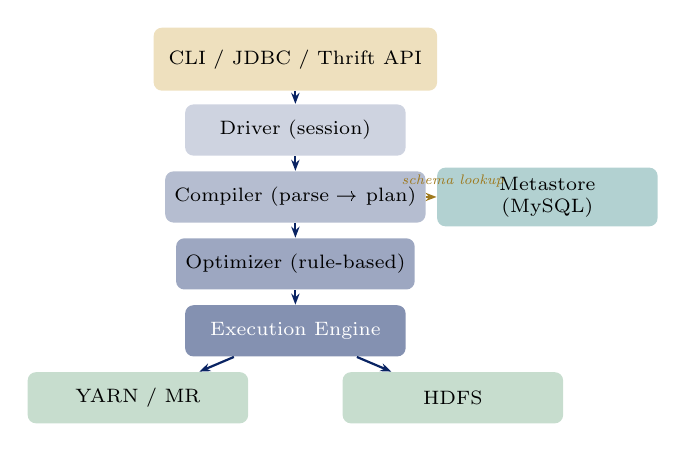
\begin{tikzpicture}[
          hbx/.style={rectangle, rounded corners=3pt, minimum width=2.8cm,
                      minimum height=0.65cm, align=center, font=\scriptsize},
          arr/.style={-{Stealth[length=4pt]}, draw=PUNavy, thick},
          darr/.style={-{Stealth[length=4pt]}, draw=PUGold!80!black,
                       thick, dashed}
        ]
        \node[hbx, fill=PUGold!30, minimum width=3.6cm, minimum height=0.8cm]
              (cli) at (0, 4.4) {CLI / JDBC / Thrift API};

        \node[hbx, fill=PUNavy!20] (drv)  at (0, 3.5) {Driver (session)};
        \node[hbx, fill=PUNavy!30] (cmp)  at (0, 2.65)
              {Compiler (parse \textrightarrow{} plan)};
        \node[hbx, fill=PUNavy!40] (opt)  at (0, 1.8)
              {Optimizer (rule-based)};
        \node[hbx, fill=PUNavy!50, text=white] (exe) at (0, 0.95)
              {Execution Engine};

        \node[hbx, fill=PUGreen!25] (mr)  at (-2.0, 0.1) {YARN / MR};
        \node[hbx, fill=PUGreen!25] (hdfs)at (2.0,  0.1) {HDFS};
        \node[hbx, fill=PUTeal!30]  (meta)at (3.2,  2.65) {Metastore\\(MySQL)};

        \draw[arr]  (cli) -- (drv);
        \draw[arr]  (drv) -- (cmp);
        \draw[arr]  (cmp) -- (opt);
        \draw[arr]  (opt) -- (exe);
        \draw[arr]  (exe) -- (mr);
        \draw[arr]  (exe) -- (hdfs);
        \draw[darr] (cmp.east) -- (meta.west);
        \node[font=\tiny\itshape, text=PUGold!80!black] at (2.0, 2.85)
              {schema lookup};
      \end{tikzpicture}
      \end{center}
  \end{columns}
\end{frame}

%----------------------------------------------------------------
\begin{frame}{Technical Contribution 2 — Metastore \& SerDe}
  \begin{columns}[T]
    \column{0.50\textwidth}
      \begin{block}{Metastore: Schema-on-Read Catalogue}
        The Hive Metastore stores:
        \begin{itemize}
          \item \textbf{Table definitions}: column names, types,
                location in HDFS, file format, compression codec
          \item \textbf{Partition metadata}: for a table partitioned
                on \texttt{(dt, country)}, the Metastore holds the
                HDFS path for each $(dt, country)$ value pair;
                enables partition pruning without listing all files
          \item \textbf{Bucket count}: number of buckets per partition;
                used to decide whether a sort-merge join avoids a shuffle
          \item \textbf{Column statistics}: NDV, min/max, nulls;
                used by cost-based optimizer (Hive 0.14+, 2015)
        \end{itemize}
      \end{block}
      \vspace{4pt}
      \begin{alertblock}{Schema-on-Read}
        Hive does \textbf{not} validate data at write time.
        A corrupt row returns \texttt{NULL} at query time.
        This allows \emph{any} file already on HDFS to be
        queried — just register a SerDe that can parse it.
      \end{alertblock}

    \column{0.47\textwidth}
      \begin{block}{SerDe: Pluggable Format Layer}
        A \textbf{SerDe} (Serializer / Deserializer) translates
        raw bytes on HDFS into Hive rows and back.
        \renewcommand{\arraystretch}{1.2}
        \begin{tabular}{@{}ll@{}}
          \toprule
          \textbf{SerDe} & \textbf{Format} \\
          \midrule
          LazySimpleSerDe & \texttt{\textbackslash{}t}-delimited text \\
          OpenCSVSerDe    & RFC 4180 CSV \\
          JsonSerDe       & JSON (one object/line) \\
          AvroSerDe       & Avro binary + schema \\
          ParquetHiveSerDe& Columnar Parquet \\
          OrcSerDe        & Columnar ORC \\
          RegexSerDe      & Any log via regex \\
          \bottomrule
        \end{tabular}
      \end{block}
      \vspace{4pt}
      \begin{exampleblock}{UDFs: Arbitrary Extension}
        Hive supports \textbf{UDF} (scalar), \textbf{UDAF} (aggregate),
        and \textbf{UDTF} (table-generating, e.g.\ \texttt{explode()}).
        Facebook registered $>$700 internal UDFs by 2010.
      \end{exampleblock}
  \end{columns}
\end{frame}

%================================================================
\section{Paper 2 — Thusoo et al.\ (2010): Hive at Petabyte Scale}
%================================================================

%----------------------------------------------------------------
\begin{frame}{Thusoo et al.\ (2010): ICDE and Production Results}
  \begin{columns}[T]
    \column{0.53\textwidth}
      \begin{paperbox}{Full Citation}
        Thusoo, A., Sarma, J.~S., Jain, N., Shao, Z., Chakka, P.,
        Zhang, N., Antony, S., Liu, H., \& Murthy, R. (2010).
        \textbf{Hive: A Petabyte Scale Data Warehouse Using Hadoop.}
        In \textit{Proceedings of the 26th IEEE International Conference
        on Data Engineering (ICDE)}, pp.~996--1005. Long Beach, CA.\\[5pt]
        \textbf{Venue:} IEEE ICDE 2010 — Rank A (CORE)\\
        \textbf{Cited by:} $>$1{,}500 (Google Scholar, 2024)\\
        \textbf{Extends}: Thusoo et al.\ 2009 with Facebook's
        production Hive deployment at petabyte scale
      \end{paperbox}
      \vspace{5pt}
      \begin{block}{New Contributions Over the 2009 Paper}
        \begin{itemize}
          \item Detailed \textbf{query optimisation} techniques:
                map-side aggregation, skew join handling,
                and multi-group-by optimisation
          \item \textbf{Index support}: compact and bitmap indexes
                for selective query speedup
          \item \textbf{Column statistics} collection (\texttt{ANALYZE TABLE})
                to guide query optimizer decisions
          \item Production benchmarks on Facebook's 2~PB cluster:
                7{,}500+ HiveQL queries/day with $<$15\% failure rate
        \end{itemize}
      \end{block}

    \column{0.44\textwidth}
      \begin{alertblock}{Facebook Production Scale (2010)}
        \renewcommand{\arraystretch}{1.25}
        \begin{tabular}{@{}ll@{}}
          \toprule
          \textbf{Metric} & \textbf{Value} \\
          \midrule
          Data stored        & 2 PB \\
          Daily growth       & 15 TB \\
          Daily queries      & 7{,}500+ \\
          Active Hive users  & 200+ analysts \\
          Longest query      & 48 hours \\
          Most used feature  & Partitioning \\
          \bottomrule
        \end{tabular}
      \end{alertblock}
      \vspace{5pt}
      \begin{exampleblock}{Key Optimization: Map-Side Aggregation}
        For \texttt{SELECT country, COUNT(*) FROM logs GROUP BY country},
        Hive performs a \textbf{partial aggregation in the mapper}
        (combiner pattern) before shuffling.
        On a 50-million-row table with 200 countries, this reduces
        shuffle data by $\approx$250{,}000$\times$.
      \end{exampleblock}
  \end{columns}
\end{frame}

%----------------------------------------------------------------
\begin{frame}{HiveQL Query Lifecycle — From SQL to MapReduce}
  \begin{columns}[T]
    \column{0.50\textwidth}
      \begin{block}{Example: Partitioned Join Query}
        \begin{semiverbatim}
\scriptsize
SELECT u.country, COUNT(*) AS plays
FROM   play\_events p
JOIN   users u ON p.user\_id = u.user\_id
WHERE  p.dt = '2024-10-01'
  AND  p.country IN ('BD','IN','US')
GROUP BY u.country
ORDER BY plays DESC;
        \end{semiverbatim}
      \end{block}
      \vspace{5pt}
      \begin{block}{Compiler Steps}
        \begin{enumerate}
          \item \textbf{Parse}: HiveQL $\to$ AST
          \item \textbf{Semantic Analysis}: resolve \texttt{p.user\_id}
                to \texttt{play\_events.user\_id : BIGINT};
                check \texttt{dt} is a partition column
          \item \textbf{Logical Plan}: Filter $\to$ HashJoin $\to$
                GroupBy $\to$ OrderBy
          \item \textbf{Partition Pruning}: only load
                \texttt{dt=2024-10-01/country=BD/},
                \texttt{.../IN/}, \texttt{.../US/}
                (skip all other 365 $\times$ 200 partitions)
          \item \textbf{Physical Plan}: MR Job~1 (join) + MR Job~2
                (global sort by \texttt{plays})
        \end{enumerate}
      \end{block}

    \column{0.47\textwidth}
      \begin{center}
      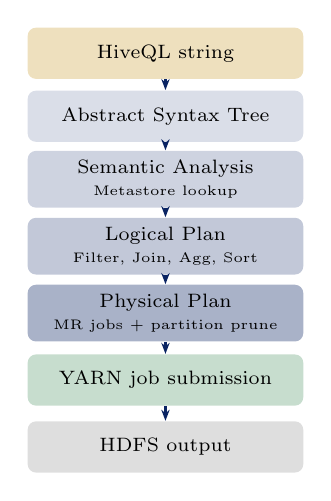
\begin{tikzpicture}[
          sb/.style={rectangle, rounded corners=3pt, minimum width=3.5cm,
                     minimum height=0.65cm, align=center, font=\scriptsize},
          arr/.style={-{Stealth[length=4pt]}, draw=PUNavy, thick}
        ]
        \node[sb, fill=PUGold!30]   (sql)  at (0, 5.2) {HiveQL string};
        \node[sb, fill=PUNavy!15]   (ast)  at (0, 4.4) {Abstract Syntax Tree};
        \node[sb, fill=PUNavy!20]   (sem)  at (0, 3.6)
              {Semantic Analysis\\{\tiny Metastore lookup}};
        \node[sb, fill=PUNavy!25]   (lp)   at (0, 2.75)
              {Logical Plan\\{\tiny Filter, Join, Agg, Sort}};
        \node[sb, fill=PUNavy!35]   (pp)   at (0, 1.9)
              {Physical Plan\\{\tiny MR jobs + partition prune}};
        \node[sb, fill=PUGreen!25]  (exec) at (0, 1.05)
              {YARN job submission};
        \node[sb, fill=PUGray!20]   (out)  at (0, 0.2) {HDFS output};

        \draw[arr] (sql)  -- (ast);
        \draw[arr] (ast)  -- (sem);
        \draw[arr] (sem)  -- (lp);
        \draw[arr] (lp)   -- (pp);
        \draw[arr] (pp)   -- (exec);
        \draw[arr] (exec) -- (out);
      \end{tikzpicture}
      \end{center}
  \end{columns}
\end{frame}

%----------------------------------------------------------------
\begin{frame}{Impact Today — Thusoo et al.\ (2009, 2010)}
  \begin{columns}[T]
    \column{0.50\textwidth}
      \begin{block}{Hive's Lasting Contributions}
        \begin{itemize}
          \item \textbf{Hive Metastore} became the de facto standard
                catalogue for all Hadoop-ecosystem tools:
                Spark, Presto/Trino, Impala all read from it
          \item \textbf{ORC format} (2013): Hive team developed
                Optimized Row Columnar; 2--4$\times$ faster reads than
                SequenceFile; predicate pushdown within stripes
          \item \textbf{LLAP} (Live Long and Process, 2016):
                Hive-on-Tez with persistent in-memory daemon;
                sub-second interactive queries on multi-TB tables
          \item \textbf{Hive-on-Spark} (2015): execution engine
                swapped from MR to Spark; same HiveQL, faster execution
          \item \textbf{AWS Glue Catalog}: managed Metastore-compatible
                API used by Athena, EMR, and Redshift Spectrum
          \item \textbf{Apache Iceberg REST Catalog}: replaces Metastore
                for next-generation lakehouse architectures
        \end{itemize}
      \end{block}

    \column{0.47\textwidth}
      \begin{exampleblock}{Stanford CS246 / CMU 15-721 Perspective}
        \begin{itemize}
          \item CMU 15-721 presents Hive as the first
                \textbf{declarative interface over a distributed
                execution engine} — separating the \emph{what}
                (HiveQL) from the \emph{how} (MR DAG).
                The same separation reappears in Spark SQL's
                Catalyst and Presto's connector model.
          \item Stanford CS246 uses Hive as a benchmark baseline
                for \textbf{join optimisation}: when to broadcast
                a small table (map-side join) vs.\ sort-merge join
                vs.\ hash join — a question that drives Presto's
                cost-based optimizer decisions
        \end{itemize}
      \end{exampleblock}
      \vspace{4pt}
      \begin{alertblock}{CLO3/CLO4 Connection}
        Hive's partition pruning + cost-based join selection
        is the canonical CLO4 \emph{problem-solving} exercise:
        design the partitioning scheme that minimises data scanned.
      \end{alertblock}
  \end{columns}
\end{frame}

%================================================================
\section{Case Study — Spotify Discover Weekly (2015--2018)}
%================================================================

%----------------------------------------------------------------
\begin{frame}{Spotify's Data Challenge}
  \begin{columns}[T]
    \column{0.52\textwidth}
      \begin{block}{Scale of the Music Listening Graph}
        Spotify (founded 2006, 75M users by 2015) generates:
        \begin{itemize}
          \item \textbf{Streaming events}: every song play, skip,
                pause, repeat, and playlist add logged as a Kafka event
                — $\approx$3 billion events per day
          \item \textbf{30 million songs} in the catalogue;
                each with audio features (tempo, key, danceability,
                acousticness) computed by audio ML models
          \item \textbf{2 billion user-created playlists}:
                implicit feedback on what songs belong together
          \item All event data landed on HDFS via Kafka consumers
                and queried daily via HiveQL for product analytics,
                A/B testing, and recommendation training
        \end{itemize}
      \end{block}
      \vspace{4pt}
      \begin{exampleblock}{Luigi: Spotify's Workflow Scheduler}
        Spotify open-sourced \textbf{Luigi} (Python, 2012) to
        orchestrate dependent HiveQL + Spark jobs as DAGs.
        A Luigi task declares its \textbf{output} (an HDFS path)
        and its \textbf{input dependencies} (other Luigi tasks).
        Luigi skips tasks whose output already exists —
        enabling incremental daily pipelines.
      \end{exampleblock}

    \column{0.45\textwidth}
      \begin{center}
      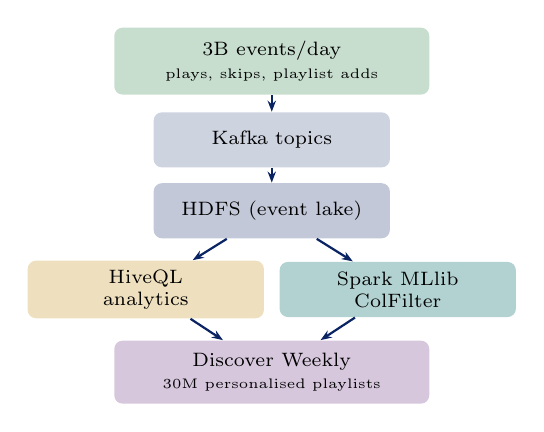
\begin{tikzpicture}[
          sp/.style={rectangle, rounded corners=3pt, minimum width=3.0cm,
                     minimum height=0.7cm, align=center, font=\scriptsize},
          arr/.style={-{Stealth[length=4pt]}, draw=PUNavy, thick}
        ]
        \node[sp, fill=PUGreen!25, minimum width=4.0cm, minimum height=0.85cm]
              (ev) at (0, 4.5)
              {3B events/day\\{\tiny plays, skips, playlist adds}};

        \node[sp, fill=PUNavy!20]  (kaf) at (0, 3.5) {Kafka topics};
        \node[sp, fill=PUNavy!25]  (hdfs)at (0, 2.6) {HDFS (event lake)};

        \node[sp, fill=PUGold!30]  (hive)at (-1.6, 1.6) {HiveQL\\analytics};
        \node[sp, fill=PUTeal!30]  (sp2) at (1.6,  1.6) {Spark MLlib\\ColFilter};

        \node[sp, fill=PUPurple!25, minimum width=4.0cm, minimum height=0.8cm]
              (dw) at (0, 0.55)
              {Discover Weekly\\{\tiny 30M personalised playlists}};

        \draw[arr] (ev)   -- (kaf);
        \draw[arr] (kaf)  -- (hdfs);
        \draw[arr] (hdfs) -- (hive);
        \draw[arr] (hdfs) -- (sp2);
        \draw[arr] (hive) -- (dw);
        \draw[arr] (sp2)  -- (dw);
      \end{tikzpicture}
      \end{center}
  \end{columns}
\end{frame}

%----------------------------------------------------------------
\begin{frame}{Discover Weekly: The Recommendation Pipeline}
  \begin{columns}[T]
    \column{0.52\textwidth}
      \begin{block}{Three-Signal Collaborative Filtering}
        Discover Weekly (launched July 2015) combines three data
        sources, all prepared via HiveQL on Hive + Spark:
        \begin{enumerate}
          \item \textbf{Playlist co-occurrence} (implicit feedback):\\
                If songs A and B appear together in $>$N playlists,
                they are ``similar.''
                \textbf{HiveQL query}:
                \texttt{SELECT song\_a, song\_b, COUNT(*) FROM}
                \texttt{playlist\_songs GROUP BY song\_a, song\_b
                HAVING COUNT(*) > 5}\\
                Over \textbf{2 billion playlists} on Hive.
          \item \textbf{NLP on artist metadata} (Natural Language Processing
                on music blog text) — \textbf{Word2Vec} on
                song co-occurrence sequences, like word2vec on sentences.
          \item \textbf{Audio feature similarity} — CNN-derived
                embeddings for 30-million songs; cosine similarity
                via Spotify's \textbf{Annoy} library.
        \end{enumerate}
      \end{block}

    \column{0.45\textwidth}
      \begin{block}{Scale Numbers (2015--2016)}
        \renewcommand{\arraystretch}{1.25}
        \begin{tabular}{@{}ll@{}}
          \toprule
          \textbf{Metric}              & \textbf{Value} \\
          \midrule
          Weekly listeners served      & 30 million \\
          Playlists analysed           & 2 billion \\
          Songs in catalogue           & 30 million \\
          Song-pair co-occurrences     & $>$1 trillion \\
          HiveQL query for co-occur.   & $\sim$2 hours \\
          Spark ALS matrix size        & 75M $\times$ 30M \\
          Weekly pipeline run time     & $\sim$24 hours \\
          User retention uplift        & $+$40\% playlist saves \\
          \bottomrule
        \end{tabular}
      \end{block}
      \vspace{4pt}
      \begin{alertblock}{Luigi DAG}
        The pipeline ran as a \textbf{Luigi DAG}:
        \texttt{CoOccurrenceHive} $\to$
        \texttt{ALSModel (Spark)} $\to$
        \texttt{TopKRecs} $\to$
        \texttt{PlaylistExporter}.
        Monday midnight trigger; playlists ready by Monday morning.
      \end{alertblock}
  \end{columns}
\end{frame}

%----------------------------------------------------------------
\begin{frame}{Lessons Learned \& Discussion Questions}
  \begin{columns}[T]
    \column{0.52\textwidth}
      \begin{block}{Key Lessons from Spotify's Case}
        \begin{enumerate}
          \item \textbf{Implicit feedback at scale beats ratings}:
                Spotify's 2 billion playlists were richer signal than
                explicit star ratings (cf.\ Netflix Prize); collecting
                behavioural events via Kafka + HDFS is the enabling
                infrastructure
          \item \textbf{HiveQL for feature engineering, Spark for ML}:
                co-occurrence aggregation (SQL) and ALS matrix
                factorisation (iterative) suit different engines;
                a single pipeline tool (Luigi) bridges them
          \item \textbf{Schema design determines query speed}:
                partitioning \texttt{play\_events} by \texttt{week}
                reduced the co-occurrence HiveQL from 8 hours to 2 hours
          \item \textbf{Cold-start is still hard}:
                new songs with no playlist appearances get audio-feature
                recommendations only; quality lags until co-occurrence
                data accumulates
          \item \textbf{Freshness vs.\ accuracy}: weekly re-training was
                a business compromise — daily retraining costs $7\times$
                the compute; monthly is too stale for trending songs
        \end{enumerate}
      \end{block}

    \column{0.45\textwidth}
      \begin{alertblock}{Discussion Questions \textmd{\tiny (CLO3, CLO4)}}
        \begin{enumerate}
          \item Spotify's co-occurrence query runs
                \texttt{GROUP BY song\_a, song\_b} over 2~billion
                playlist rows.
                Estimate the output size if there are 30M songs.
                Propose a \textbf{partitioning + bucketing} scheme
                for the \texttt{playlist\_songs} Hive table that
                would reduce the shuffle size for this query.
                \textit{[CLO4 — Apply]}
          \item The ALS collaborative filtering model is a matrix
                factorisation over a 75M-user $\times$ 30M-song matrix.
                At 4 bytes per float and rank $k=50$, calculate
                the model size and explain whether it fits in a
                5{,}000-node YARN cluster's aggregate RAM.
                \textit{[CLO4 — Analyse]}
          \item Spotify uses \textbf{Luigi} while other companies
                use \textbf{Apache Airflow}.
                Compare the two on: dependency declaration style,
                backfill capability, and UI/observability.
                Which would you choose for a 100-step daily pipeline?
                \textit{[CLO3 — Evaluate]}
        \end{enumerate}
      \end{alertblock}
  \end{columns}
\end{frame}

%================================================================
\section{Live Exercise}
%================================================================

%----------------------------------------------------------------
\begin{frame}[fragile]{Live Exercise — HiveQL on Local Hadoop (or SparkSQL)}
  \begin{columns}[T]
    \column{0.50\textwidth}
      \begin{block}{Task (25 minutes, pairs)}
        Simulate a Hive session using \textbf{PySpark's SQL interface}
        (which reads the same Hive Metastore).\\[5pt]
        \textbf{Dataset}: a 10{,}000-row synthetic \texttt{play\_events}
        CSV (generate with the skeleton below).\\[5pt]
        \textbf{Goals}:
        \begin{enumerate}\setlength\itemsep{1pt}
          \item Create a partitioned Spark table
                (partition on \texttt{dt}).
          \item Run the co-occurrence query and time it.
          \item Add a \textbf{broadcast join} hint for the
                \texttt{songs} dimension table and compare timings.
          \item Use \texttt{EXPLAIN} to print the physical plan
                and identify where partition pruning occurs.
        \end{enumerate}
      \end{block}

    \column{0.47\textwidth}
      \begin{exampleblock}{PySpark SQL Skeleton}
        \scriptsize
        \begin{verbatim}
from pyspark.sql import SparkSession
import random, datetime

spark = SparkSession.builder \
        .appName("HiveDemo") \
        .getOrCreate()
spark.setLogLevel("WARN")

# Generate synthetic data
rows = []
for i in range(10_000):
    rows.append({
      "user_id":    random.randint(1, 500),
      "song_id":    random.randint(1, 200),
      "playlist_id":random.randint(1, 1000),
      "dt":         "2024-10-01"
    })

df = spark.createDataFrame(rows)
df.createOrReplaceTempView("play_events")

# Co-occurrence query
result = spark.sql("""
  SELECT a.song_id AS song_a,
         b.song_id AS song_b,
         COUNT(*)  AS co_count
  FROM   play_events a
  JOIN   play_events b
    ON   a.playlist_id = b.playlist_id
   AND   a.song_id < b.song_id
  GROUP BY a.song_id, b.song_id
  HAVING COUNT(*) > 2
  ORDER BY co_count DESC
""")
result.show(10)
        \end{verbatim}
      \end{exampleblock}
  \end{columns}
\end{frame}

%================================================================
\section*{References}
%================================================================

%----------------------------------------------------------------
\begin{frame}{References}
  \begin{block}{Seminal Papers}
    \begin{itemize}
      \item Thusoo, A., et al. (2009).
            Hive: A warehousing solution over a map-reduce framework.
            \textit{Proc.\ VLDB Endowment, 2}(2), 1626--1629.
      \item Thusoo, A., et al. (2010).
            Hive: A petabyte scale data warehouse using Hadoop.
            \textit{Proc.\ IEEE ICDE}, 996--1005.
    \end{itemize}
  \end{block}
  \vspace{4pt}
  \begin{block}{Textbooks \textmd{[TW], [SA], [TE]}}
    \begin{itemize}
      \item \textbf{[TW]} White, T. (2015).
            \textit{Hadoop: The Definitive Guide}, 4th ed.
            (Ch.~17 — Hive). O'Reilly.
      \item \textbf{[SA]} Acharya, S., \& Chellappan, S. (2015).
            \textit{Big Data and Analytics}
            (Ch.~7 — Data Warehousing on Hadoop). Wiley.
      \item \textbf{[TE]} Erl, T., Khattak, W., \& Buhler, P. (2016).
            \textit{Big Data Fundamentals}
            (Ch.~9 — SQL-on-Hadoop). Prentice Hall.
    \end{itemize}
  \end{block}
  \vspace{4pt}
  \begin{block}{Case Study Sources}
    \begin{itemize}
      \item Spotify Engineering. (2015).
            \textit{How Spotify Discover Weekly Works}.
            labs.spotify.com/2015/08/06.
      \item Kula, E. (2015).
            \textit{From Idea to Execution: Spotify's Discover Weekly}.
            Spotify R\&D blog.
    \end{itemize}
  \end{block}
\end{frame}

%----------------------------------------------------------------
\begin{frame}{Closing — Week 7, Part 2}
  \begin{columns}[T]
    \column{0.52\textwidth}
      \begin{block}{Key Takeaways}
        \begin{itemize}
          \item Thusoo et al.\ (2009) gave the world a
                \textbf{declarative interface over distributed storage}
                — HiveQL's impact was democratisation:
                200 analysts replaced 20 Java engineers
          \item The \textbf{Metastore} is Hive's most durable
                contribution — it outlived MR-based Hive execution
                and is now the universal catalogue for Spark, Presto,
                Trino, Athena, and Delta Lake
          \item Spotify's case demonstrates that
                \textbf{SQL (HiveQL) and iterative ML (Spark ALS)}
                are complementary in a recommendation pipeline —
                neither alone is sufficient at billion-playlist scale
          \item \textbf{Schema design is a first-class skill}:
                the right partition column (week vs.\ song vs.\ user)
                changes query latency by hours on petabyte data
        \end{itemize}
      \end{block}

    \column{0.45\textwidth}
      \begin{alertblock}{Quote of the Week}
        \begin{center}
        \large\itshape
        ``Hive provides a simple and optimizable
        query language, familiar to all
        data warehouse users, while
        retaining the scalability of Hadoop.''
        \end{center}
        \begin{flushright}
        \small --- Thusoo et al.\ (2009)
        \end{flushright}
      \end{alertblock}
      \vspace{6pt}
      \begin{exampleblock}{Part 1 Preview — Week 8}
        \textbf{Kafka, Sqoop, Flume, Lambda/Kappa Architecture}\\[3pt]
        \begin{itemize}\setlength\itemsep{1pt}
          \item Kafka topics, partitions, consumer groups
          \item Exactly-once semantics
          \item Lambda: batch + speed + serving layers
          \item Kappa: stream-only simplification
        \end{itemize}
      \end{exampleblock}
  \end{columns}
\end{frame}

%=================================================================
\end{document}
%=================================================================
